
From here, we can relate PM magnetic field to air gap magnetic field as $H_{PM} = -\frac{H_{\delta}\delta}{h_{PM}}$. Here, negative sign suggests the fields at the air gap and on PM are opposing to each other. Magnetic field on the PM opposing the PM magnetizing direction is called demagnetizing field, explained in Sec. \ref{sec:demagnetizingField}.

\begin{figure}[h]
    \centering
    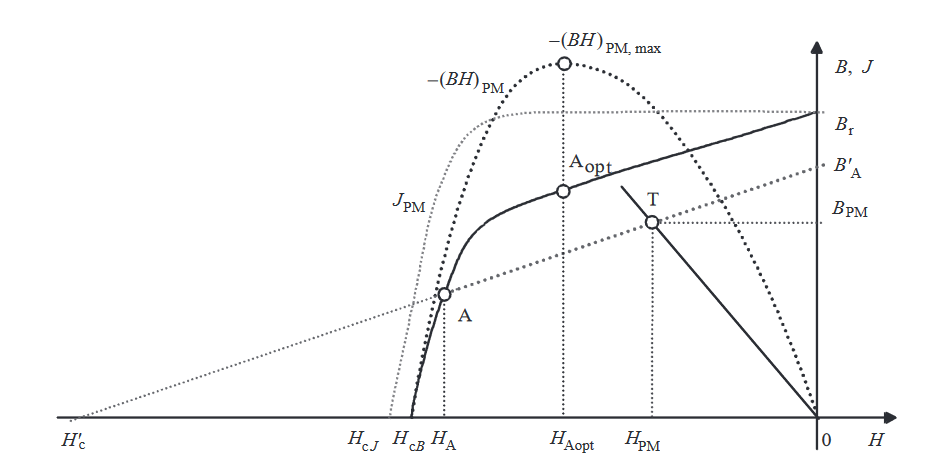
\includegraphics[width=1.00\textwidth]{2ndquarter.png}
    \label{fig:2ndquarter}
\end{figure}

In addition to Eq. \ref{eq:Ampereslaw_magcircapp}, $H_{\delta}$ can be written as

\begin{equation}
	H_{\delta} = B_{\delta}/\mu_{0}	
\end{equation}

where, $B_{\delta}$ is air gap magnetic flux density. Considering a uniform ring structure, where cross-section area of PM and air gap is equal $A_{PM} = A_{\delta}$ and assuming no leakage flux in the system, air gap magnetic flux density equals to PM magnetic flux density $B_{PM} = B_{\delta}$. Furthermore, PM magnetic flux density $B_{PM}$ is related to the demagnetizing field $H_{PM}$ by

\begin{figure}[h]
    \centering
    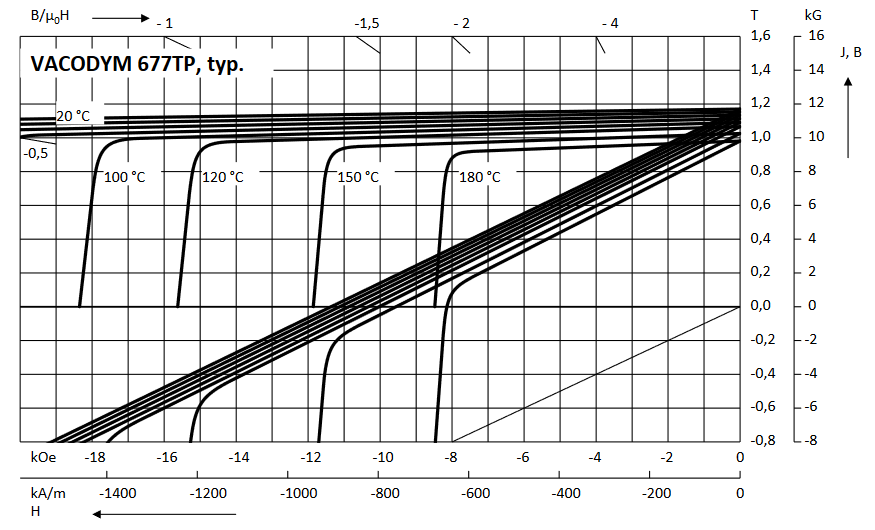
\includegraphics[width=0.35\textwidth]{vac677TP.png}
    \label{fig:vac677TP}
\end{figure}

\begin{eqnarray}
	B_{PM} = B_{r} + \mu_{0}\mu_{r}H_{PM}
\end{eqnarray}

then, Eq. \ref{eq:Ampereslaw_magcircapp} becomes

\begin{equation}
	\frac{B_{r}}{u_{r}} = (\frac{1}{\mu_{r}}+\frac{\delta}{h_{PM}})B_{PM}
\end{equation}

describing magnetic flux density supplied by the PM in relation with the PM and air gap lengths. Moreover, arranging Eq. \ref{eq:Ampereslaw_magcircapp}

\begin{eqnarray}
	H_{\delta} = -\frac{H_{PM}h_{PM}}{\delta} \\
	\mu_{0}	H_{\delta} = -\mu_{0} \frac{H_{PM}h_{PM}}{\delta} \\
	B_{PM} = B_{\delta} = \mu_{0} H_{\delta} \\
	\frac{B_{PM}}{H_{PM}} = -\mu_{0} \frac{h_{PM}}{\delta}
\end{eqnarray}

which constitutes the load line $0-T$ at no-load $NI = 0$. Let's increase the air gap length slowly, starting from an initial value of $\delta = 0$. As air gap length increases, operating point moves along the curve at \nth{2} quadrant, starting from point $B_{r}$. As the air gap length $\delta$ increases, demagnetizing field increases as well. At a certain point $H = H_{Aopt}$, the energy stored in the PM becomes highest as $|BH|$ becomes maximum. At a higher demagnetizing field of $H_{A}$, operating point moves along what it seem to be a 'knee' on Fig. \ref{fig:2ndquarter}. If the operating point does not pass this 'knee', then the operation is reversible, meaning that as the demagnetizing field lowers, the operating point moves back on the same curve. However, if the operating point does not pass this 'knee' as in the case where operating point is at point $A$, then the operation is irreversible. A new recoil curve, $A-B'_{A}$, is drawn. Hereafter, the remanent flux density is $B'_{A}$, lower than $B_{r}$.



It is clear that as air gap length increases, PM flux density decreases. Also, the demagnetizing curve has a slope of $\mu_{0} \mu_{r}$. What this indicates is that PM operation over reversible demagnetizing curve does not solely consists of external field, but there are processes going on within the PM material. These processes are a combination of magnetization rotation (reversible) and Barkhausen jumps (irreversible, causes hysteresis).

  If air gap length exceeds some level such that the resulting demagnetizing field on the PM surpasses the level that correspond to the knee point (point where the slope of the curve increases abruptly), then the magnet is irreversibly demagnetized. Without a load acting on the magnetic circuit, this kind of a demagnetization in PM is highly unlikely.
  Equation for load line is given as
\begin{equation}
	\frac{B_{m}}{H_{m}} = -\mu_{0} \frac{A_{g}}{A_{m}} \frac{l_{m}}{l_{g}}
\end{equation}

